\chapter{Theory}
\label{ch:theory}

\section{Model: Sequential}
\label{sec:sequentialmodel}

\begin{figure}[ht]
	\centering
	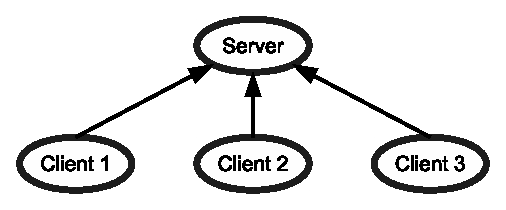
\includegraphics[width=0.45\linewidth]{sequentialmodel}
	\caption{Sequential model}
	\label{fig:sequentialmodel}
\end{figure}

In the sequential (client\,/\,server) model, as shown in figure \ref{fig:sequentialmodel}, every client is only connected to the server. The server transfers data sets to all clients in parallel. These peers share the upload bandwidth of the server. This concept does not scale well, because every new client connecting to the system slows down every other client connected to the same server. 

To estimate the efficiency of this model, let $b$ the bandwidth of the server in $\frac{bytes}{seconds}$, $n$ the number of clients connected to the server and $s$ the size of the whole data set in bytes. Then $T= n\:T_0$ is the time in seconds it takes to transfer the data set to all clients, where $T_0=\frac{s}{b}$ is the time in seconds for a single transfer from the server to a client. To fulfill this formula, each client needs at least as much download bandwidth as the shared upload bandwidth of the server. Without adding more servers or using the upload bandwidth of the clients this linear relationship can not be removed. The implementation of this model is explained in section \ref{subsubsec:seqlog} and is obviously not able to keep the limit of $2\:T_0$ seconds, but it has been implemented to show the immense difference. A more efficient approach is presented in section \ref{sec:logarithmicmodel}.

\pagebreak
\section{Model: Logarithmic}
\label{sec:logarithmicmodel}

\begin{figure} [ht]
	\centering
	\begin{minipage}[b]{0.4\linewidth}
		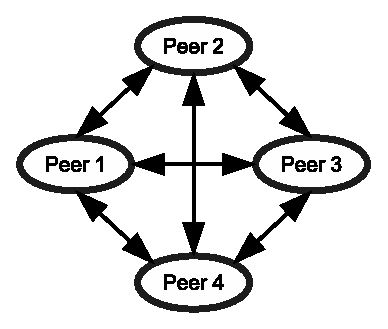
\includegraphics[width=\textwidth]{peermesh}
		\caption{Peer mesh}
		\label{fig:peermesh}
	\end{minipage}
	\hspace{0.1\linewidth}
	\begin{minipage}[b]{0.4\linewidth}
		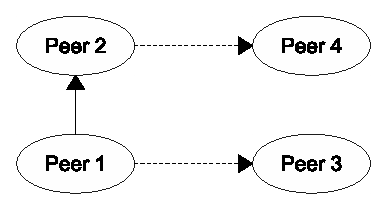
\includegraphics[width=\textwidth]{logarithmicmodel}
		\caption{Logarithmic model}
		\label{fig:logarithmicmodel}
	\end{minipage}

\end{figure}


If a Peer-to-Peer model is used instead of the Sequential model, every so called peer is connected to one or more other peers depending on the used topology. In this thesis only the mesh topology is of importance, as shown in figure \ref{fig:peermesh}, where every peer is connected to every other peer in the network.

In the Logarithmic model every peer can do both uploading and downloading data sets, though peers are restricted to only upload to one other peer in parallel. If a new data set is announced by one peer in the Peer-to-Peer network, all peers try to download this data set from the given peer. Only one peer, basically the fastest one, is allowed to download the data set. The rest of the requesting peers are rejected and do nothing while the other peers download the data set. When the peer completed the download, the number of peers containing the data set changes to two. This time another two peers will be allowed to download the data set. Therefore, the number of downloading peers doubles periodically, which is considered exponential growth.

This model guarantees, that every peer has the complete data set in $T=\log_{2}{(n)}\:T_0$  seconds, where $n$ is the number of peers in the network, $T_0=\frac{s}{u}$ the time for a single transfer from one peer to another, $s$ the size of the data set and $u$ the upload bandwidth of each peer. This is only true for peers with a higher download bandwidth than upload bandwidth and applies to all Peer-to-Peer models presented in this chapter. In reality this makes sense, because clients connected through an \emph{ISP (Internet Service Provider)} often fulfill this condition. All peers also have the same upload bandwidth $u$. Unfortunately, this is not so common in real world situations. But it can illustrate the relationship between the upload bandwidth and the number of peers. The figure \ref{fig:logarithmicmodel} shows four peers, where peer one is the only peer with the data set at first. It transfers the data set to peer two in $T_0$ seconds. Then peer one and two transfer this data set to peer three and four in parallel, which also takes $T_0$ seconds. So the whole transfer takes $2\:T_0$ seconds.

In comparison to the Sequential model, this one increases the complexity of the implementation only marginal, but the efficiency is significantly higher. The more peers participate the higher is the efficiency. The overhead is also manageable, because during the transfers the idle peers do nothing except waiting. As a major drawback of this model, there are never more than 50\% of all peers uploading in parallel. Additionally, only one peer uploads the data set at the beginning, so for the first $T_0$ seconds no other peer is uploading. This model is implemented and explained in section \ref{subsubsec:seqlog}. Finally, this model can not always keep the $2\:T_0$ limit. An improved version of this model is presented in section \ref{sec:chunkedswarmmodel}.

\section{Model: Chunked-Swarm}
\label{sec:chunkedswarmmodel}

\begin{figure} [ht]
	\centering
	\begin{minipage}[b]{0.4\linewidth}
		\centering
		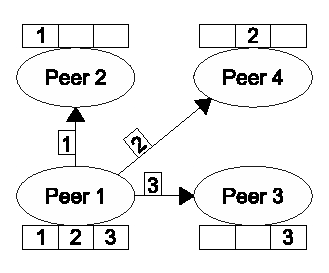
\includegraphics[width=0.7\textwidth]{chunkedswarmmodel1}
		\caption{Chunked-Swarm model 1}
		\label{fig:chunkedswarmmodel1}
	\end{minipage}
	\hspace{0.1\linewidth}
	\begin{minipage}[b]{0.4\linewidth}
		\centering
		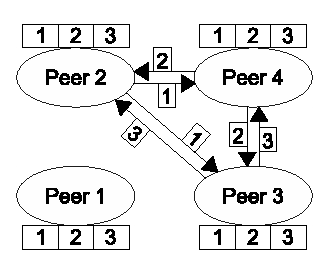
\includegraphics[width=0.7\textwidth]{chunkedswarmmodel2}
		\caption{Chunked-Swarm model 2}
		\label{fig:chunkedswarmmodel2}
	\end{minipage}
\end{figure}

\begin{figure}[ht]
	\centering
	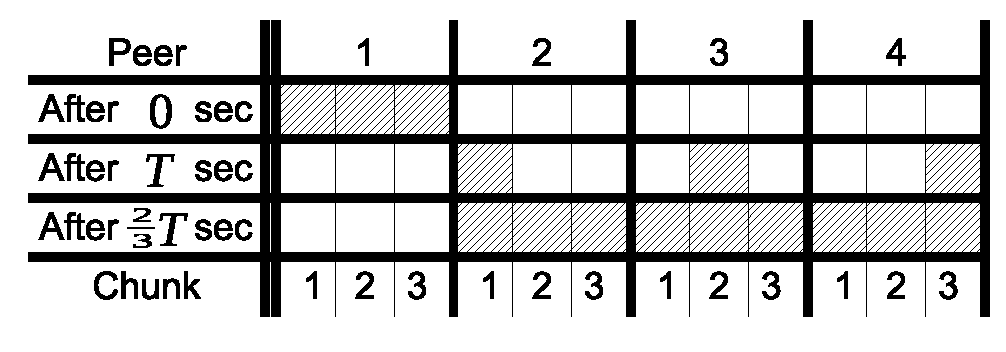
\includegraphics[width=0.8\linewidth]{chunkedswarmformula1}
	\caption{Chunked-Swarm chunk completion diagramm}
	\label{fig:chunkedswarmformula1}
\end{figure}

The Chunked-Swarm model is an enhancement of the Logarithmic model. It allows multiple uploads in parallel and splits the data set into chunks before transferring it. Therefore, peers can not download the whole data set at once. Instead, they have to request each chunk individually. Since the size of these chunks is smaller than the size of the whole data set, peers can help to distribute the data set more quickly. The figure \ref{fig:chunkedswarmmodel1} and \ref{fig:chunkedswarmmodel2} show four peers distributing three chunks. At first peer one has the data set completely. The remaining peers each request one chunk in parallel. These peers will then distribute their chunks among themselves. They do so by announcing their own chunks to all other peers they are connected with, which can then request these chunks. It is important to note, that this model is always pull-based. A chunk is only uploaded, if a peer explicitly requests it.

Compared to the Logarithmic model, the implementation of this model is more complex, because the efficiency essentially depends on the right choice of chunks the peers request from each other. Since this approach is pull-based, peers do not know, which chunks other peers request. Thus two peers may request the same chunk, which is called chunk duplication and decreases the efficiency considerably. In the context of figure \ref{fig:chunkedswarmmodel1} and \ref{fig:chunkedswarmmodel2}, chunk duplication would occur, if all peers requested chunk one from peer one. Therefore, they could not exchange this chunk afterwards. An implementation of this model has to make strong considerations about this issue. The implementation of this model is described in section \ref{subsubsec:chunkedswarm}, which also explains the problem of chunk selection in more detail. 

To determine the runtime of this model, distinct chunk selection is assumed, so there have to be at least as many chunks as peers, because otherwise chunk duplication can not be prevented. In figure \ref{fig:chunkedswarmformula1} there are just as many chunks as peers, so it takes $T_0$ seconds to transfer all distinct chunks to all peers, because every peer gets a third of the available bandwidth and also has to download a third of the whole data set. Then the peers distribute their chunks among themselves, which takes $\frac{2}{3}\:T_0$ seconds, because every peer uploads its chunk to two other peers. After $T = T_0\:+\:\frac{2}{3}\:T_0$ seconds every peer has all chunks available. Similiary a variable number of peers need $T(n) = T_0\:+\:\frac{n - 1}{n}\:T_0$ seconds. Since $0 < \frac{1}{n} \leq 1$ is always true, $T$ never exceeds $2\:T_0$. If the chunk count is doubled, the model behaves even better, because the peers can start to upload their own chunks, while they are downloading the next distinct chunks from peer one. This leads to the general formula $T(n, c) = T_0\:+\:\frac{n}{c} \cdot \frac{n-1}{n}\:T_0 = (1\:+\:\frac{n-1}{c})\:T_0$, where $c = n\:2^i, i \in \mathbb{N}_0$. As a major disadvantage, the chunk count has to be chosen before the transfer can actually happen. Since the efficiency depends on the $\frac{n-1}{c}$ ratio, the maximal number of peers should be determined before. Without any further optimizations the main objective of this thesis is already fulfilled, as long as the chunk count is equal to or greater than the peer count and no chunk duplication occurs.

If the data set is first seperated into parts, which are then segmented into chunks, the data set can be downloaded sequentially, as long as each peer downloads part after part, starting with the first part. Each part then represents a data set as well, which simplifies the implementation of this concept. One domain relying on such a download behaviour is video streaming, where peers want to watch the video while downloading it. Unfortunately, this model introduces an initial delay, because the first part has to be downloaded completely before the video can be started. The duration of the delay depends on the number of parts and chunks and on the upload and download bandwidth of each peer. Those parameters should be chosen wisely to reduce this delay as much as possible and thus to improve the quality of service. This concept is explained and implemented in section \ref{sec:streaming} and chapter \ref{ch:futurework}.

